\section{Pretrained-model audits and their boundaries}
\label{sec:experiments}

We test whether the response model remains numerically useful in trained
modules attached to real pretrained language models, how noise and query
choice affect recovery, and whether recovered coordinates improve a
structural decision. The theory supplies the global quantifiers; these
experiments do not test every feasible factorization or validate the
theorem's conservative constants. Earlier synthetic and byte-LM studies,
including large errors and failed rejection rules, remain in
Appendix~\ref{app:earlier-illustrations}.

\paragraph{Nine models, a fixed module, and held-out gradient domains.}
We use three Pythia sizes (160M, 1B, 2.8B), four dense Qwen3 sizes
(0.6B, 1.7B, 4B, 8B), and two SmolLM2 sizes (360M, 1.7B)
\citep{biderman2023pythia,yang2025qwen3,allal2025smollm2}.
Each frozen BF16 backbone receives a $K=4$ softmax-shared additive module
on 64 fixed output channels of every attention output projection. Its bases
are direct trainable matrices, not LoRA products. A fixed isometric
embedding preserves the factor-response model
(Proposition~\ref{prop:llm-embedding}). We train only these modules for
256 AdamW updates on WikiText-2, using three seeds per model and the final
checkpoint. The resulting 27 checkpoints are adapter replicates of nine
fixed pretrained models, not 27 independent pretraining runs.

Natural queries are measured next-token-loss gradients from disjoint
 general-text, MBPP code, and GSM8K math documents
\citep{merity2016wikitext,austin2021mbpp,cobbe2021gsm8k}.
The code and math domains are not used for adaptation or calibration.
Responses are controlled reverse-gradient/forward-JVP observations of the
factor map in FP64, treating the measured BF16-backbone gradients as fixed
inputs. They are not observed AdamW updates. The internal product and
matrix-valued responses are available; this is not an output-only attack.
The full protocol, model revisions, rejected access requests, development
corrections, and data/source hashes are in Appendix~\ref{app:llm-study}.

\paragraph{Finite recovery across model sizes and query types.}
We compare the repeated-complement design of
Corollary~\ref{cor:finite-noisy-main}, Gaussian queries, and three natural
 gradient families, with $q\in\{1,4,8\}$, four independent held-out
 directions, and relative noise $0,10^{-6},10^{-4},10^{-2}$ added to both
product and responses. The noisy product subspace is re-estimated and
orthogonal residuals are retained. Three estimators use observations only;
permutation-aligned ground truth is supplied afterward for scoring.

All 1,080 cases with $q\ge4$ have sufficient observed ranks and return
joint-fit factor error below $0.034$; their median error is
$1.86\times10^{-5}$. At $q=4$ without noise, the worst error across all
models and query families is $8.31\times10^{-13}$.
Table~\ref{tab:llm-models} reports maxima rather than selected seeds.
All 540 cases with $q=1$ fail the sufficient local-rank check; joint fitting
is not run and these cases count as rejected. This is the failure of the
specified reconstruction condition, not a proof that every one-query
estimator is impossible.

\begin{table}[t]
\centering\small
\caption{Joint-fit factor error with $q=4$: maxima over three adaptation seeds, and (for natural queries) three text domains. Noise affects both product and response. $D$ is the adapter basis dimension, not the backbone parameter count. Each reported maximum includes all declared cases.}
\label{tab:llm-models}
\begin{tabular}{lrrrrr}
\toprule
Model & $L$ & $D$ & Natural, $0$ & Natural, $10^{-4}$ & Designed, $10^{-4}$\\
\midrule
Pythia 160M & 12 & 49152 & $6.5\!\times\!10^{-14}$ & $1.6\!\times\!10^{-4}$ & $1.4\!\times\!10^{-4}$\\
Pythia 1B & 16 & 131072 & $2.8\!\times\!10^{-13}$ & $5.7\!\times\!10^{-5}$ & $5.7\!\times\!10^{-5}$\\
Pythia 2.8B & 32 & 163840 & $8.3\!\times\!10^{-13}$ & $3.9\!\times\!10^{-5}$ & $3.8\!\times\!10^{-5}$\\
Qwen3 0.6B & 28 & 131072 & $6.6\!\times\!10^{-14}$ & $4.9\!\times\!10^{-5}$ & $4.9\!\times\!10^{-5}$\\
Qwen3 1.7B & 28 & 131072 & $9.2\!\times\!10^{-14}$ & $4.2\!\times\!10^{-5}$ & $4.2\!\times\!10^{-5}$\\
Qwen3 4B & 36 & 262144 & $1.0\!\times\!10^{-13}$ & $3.7\!\times\!10^{-5}$ & $3.7\!\times\!10^{-5}$\\
Qwen3 8B & 36 & 262144 & $2.6\!\times\!10^{-13}$ & $3.7\!\times\!10^{-5}$ & $3.6\!\times\!10^{-5}$\\
SmolLM2 360M & 32 & 61440 & $7.8\!\times\!10^{-14}$ & $3.8\!\times\!10^{-5}$ & $3.8\!\times\!10^{-5}$\\
SmolLM2 1.7B & 24 & 131072 & $6.4\!\times\!10^{-14}$ & $4.5\!\times\!10^{-5}$ & $4.4\!\times\!10^{-5}$\\
\bottomrule
\end{tabular}
\end{table}


\begin{figure}[t]
\centering
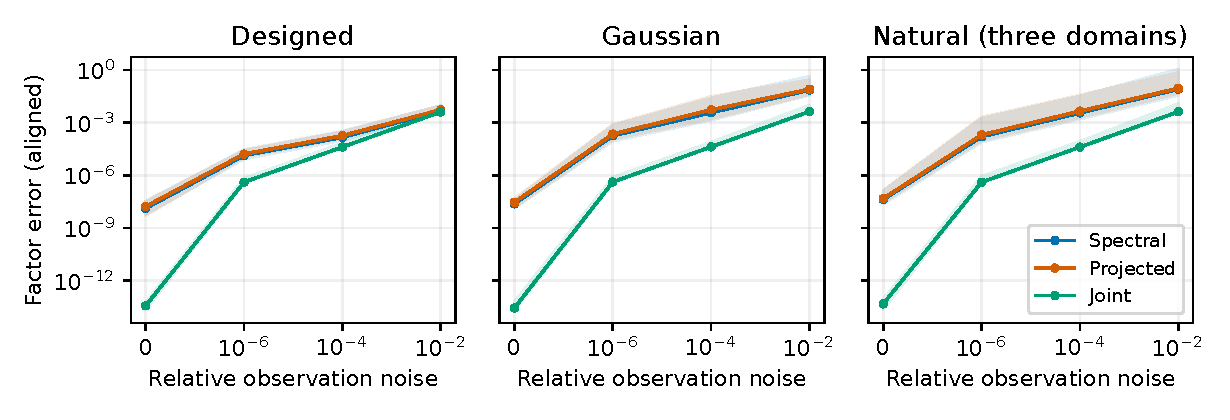
\includegraphics[width=\linewidth]{figures/llm_recovery.pdf}
\caption{Recovery with four queries. Lines show medians and shaded bands
 the 10th--90th percentiles over all 27 checkpoints; the natural panel also
includes all three domains. These are descriptive spreads across correlated
cases, not confidence intervals. Noiseless results use controlled FP64
factor responses, not full-LLM FP64 inference.}
\label{fig:llm-recovery}
\end{figure}

\paragraph{Calibration transfers here, but does not certify recovery.}
Four separate Pythia adapter checkpoints, with general-text validation
queries only, fix acceptance thresholds before held-out recovery scoring.
At error $>0.10$ defined as bad, the combined joint-fit rule accepts all
1,080 sufficient-rank cases with no observed bad output; residual-only
accepts 868, also with none. This sample therefore cannot establish better
bad-case detection by the combined rule. For projected spectral recovery,
 the combined rule accepts 43 bad outputs among 1,056, versus 20 among 1,037
for residual-only; its largest accepted error is $6.19$.
Raw spectral recovery has an all-reject calibrated policy under the strict
simplex gate, even though many of its factor errors are small.
Table~\ref{tab:llm-acceptance} retains all denominators. The earlier synthetic
study also retains a combined-rule accepted-bad fraction of $5.16\%$,
above its $5\%$ target. Neither calibration nor candidate-local diagnostics
replace the theorem's externally specified domain assumptions.

\paragraph{Precision and structural usefulness remain limiting.}
The controlled response formula agrees with autodiff within
$1.62\times10^{-16}$ relative error. Finite-step subtraction is less
reliable: at step $10^{-5}$, FP32 errors range from $0.040$ to $0.102$,
and BF16 errors from $1.00$ to $1.95$. Separately, shrinking the router-rank
margin in learned factors amplifies noisy recovery error by roughly three
orders of magnitude in the registered secondary stress test
(Figure~\ref{fig:llm-conditioning}).

On nine declared checkpoints, balanced hard groups selected from recovered
routers at noise $10^{-4}$ and $10^{-2}$ exactly reproduce the native
router partitions. However, balanced clustering of the effective parameters
also reproduces all nine. Equal-budget refitting and 64 recovery updates
 therefore provide no evidence that coordinate recovery improves this
 decision over the simpler effective-parameter control. Random balanced
 groups worsen general-text NLL after recovery at all nine checkpoints,
while code/math differences have mixed signs. These are token-loss results,
not generation accuracy or realized inference speedups. Detailed action
results, repeated-action numerical controls, costs, and independent CPU
replays are in Appendix~\ref{app:llm-study}.
